% !TEX program = xelatex
\documentclass[12pt,a4paper]{ctexart}

% ==================== 页面布局 ====================
\usepackage[top=2.5cm, bottom=2.5cm, left=2.8cm, right=2.8cm, headheight=14pt]{geometry}
\usepackage{graphicx}
\usepackage{float}
\usepackage{amsmath,amssymb}
\usepackage{listings}
\usepackage{xcolor}
\usepackage{hyperref}
\usepackage{fancyhdr}
\usepackage{booktabs}
\usepackage{enumitem}
\usepackage{titlesec}

% ==================== 代码高亮 ====================
\definecolor{codebg}{RGB}{248,248,248}
\definecolor{codeframe}{RGB}{200,200,200}
\definecolor{commentcolor}{RGB}{0,128,0}
\definecolor{keywordcolor}{RGB}{0,0,200}
\definecolor{stringcolor}{RGB}{180,60,0}
\definecolor{numbercolor}{RGB}{128,128,128}

\lstset{
    language=Python,
    basicstyle=\ttfamily\footnotesize,
    backgroundcolor=\color{codebg},
    frame=single,
    framerule=0.5pt,
    rulecolor=\color{codeframe},
    numbers=left,
    numberstyle=\tiny\color{numbercolor},
    numbersep=8pt,
    tabsize=4,
    breaklines=true,
    breakatwhitespace=false,
    showstringspaces=false,
    commentstyle=\color{commentcolor}\itshape,
    keywordstyle=\color{keywordcolor}\bfseries,
    stringstyle=\color{stringcolor},
    captionpos=t,
    xleftmargin=1.5em,
    xrightmargin=0em,
    aboveskip=1em,
    belowskip=1em,
}

% ==================== 页眉页脚 ====================
\pagestyle{fancy}
\fancyhf{}
\fancyhead[L]{\small 计算机视觉课程作业（2）：边缘检测}
\fancyhead[R]{\small 章屹倬}
\fancyfoot[C]{\thepage}
\renewcommand{\headrulewidth}{0.5pt}

% ==================== 标题格式 ====================
\titleformat{\section}{\Large\bfseries}{\thesection}{1em}{}
\titleformat{\subsection}{\large\bfseries}{\thesubsection}{1em}{}

% ==================== 文档信息 ====================
\title{\vspace{2cm}\Huge\textbf{边缘检测实验报告}\\[0.5cm]
       \Large Sobel · Laplacian · DoG · LoG · Canny}
\author{\large 章屹倬 \quad 学号：231880366}
\date{\large 2026年6月}

\begin{document}

% ==================== 封面 ====================
\maketitle
\thispagestyle{empty}

\vspace{2cm}
\begin{center}
    \large\textbf{计算机视觉课程作业（2）}\\[0.5cm]
    \normalsize 提交日期：2026年6月2日
\end{center}

\newpage

% ==================== 摘要 ====================
\thispagestyle{empty}
\begin{center}
    \Large\textbf{摘\quad 要}
\end{center}
\vspace{1cm}

本实验围绕图像边缘检测展开，使用 Python 3 与 OpenCV 4.8 实现了五种经典边缘检测算子：
Sobel（一阶梯度算子）、Laplacian（二阶导数算子）、DoG（高斯差分）、LoG（高斯拉普拉斯）和 Canny（多阶段优化算子）。
实验以 2268$\times$4032 分辨率的桥梁照片为测试图像，系统分析了各算子的检测原理、实现方式和输出特性。
结果表明：Sobel 算子能提取方向性梯度信息但边缘较粗；Laplacian 对噪声极度敏感；DoG 作为 LoG 的近似，能高效检测多尺度边缘；LoG 通过先平滑后求导的策略有效抑制了噪声干扰；Canny 凭借非极大值抑制和双阈值滞后连接，提供了最干净、最连续的边缘输出。
本实验通过对比分析，深入理解了基于导数的边缘检测方法的数学本质与工程权衡。

\vspace{1cm}
\noindent\textbf{关键词：}边缘检测；Sobel算子；拉普拉斯算子；LoG；DoG；Canny；梯度；非极大值抑制

\newpage

% ==================== 目录 ====================
\tableofcontents
\newpage

% ==================== 第一章：引言 ====================
\section{引言}

\subsection{实验背景}

边缘检测（Edge Detection）是计算机视觉中最基础的前端处理步骤之一，广泛应用于目标识别、图像分割、特征提取和三维重建等任务。边缘定义为图像中亮度发生急剧变化的像素集合，对应于一阶导数的极大值点或二阶导数的过零点。

边缘检测的核心数学工具是图像的\textbf{梯度}（gradient）。对于二维图像 $I(x,y)$，梯度向量定义为：

\begin{equation}
    \nabla I = \begin{bmatrix}
        \dfrac{\partial I}{\partial x} \\[8pt]
        \dfrac{\partial I}{\partial y}
    \end{bmatrix}
    \label{eq:gradient}
\end{equation}

梯度幅度（magnitude）反映边缘强度，梯度方向（orientation）反映边缘走向：

\begin{equation}
    |\nabla I| = \sqrt{\left(\frac{\partial I}{\partial x}\right)^2 + \left(\frac{\partial I}{\partial y}\right)^2},
    \quad
    \theta = \arctan\left(\frac{\partial I/\partial y}{\partial I/\partial x}\right)
    \label{eq:magnitude}
\end{equation}

由于数字图像是离散的，梯度通过有限差分近似计算。不同的差分模板（卷积核）对应不同的边缘检测算子。

\subsection{实验目的}

\begin{enumerate}[leftmargin=*]
    \item 掌握 Sobel、Laplacian、DoG、LoG、Canny 五种边缘检测算子的数学原理
    \item 理解一阶导数和二阶导数在边缘检测中的不同表现
    \item 理解高斯平滑在边缘检测预处理中的关键作用
    \item 对比各算子的优缺点和适用场景
    \item 培养实验结果的可视化对比与科学分析能力
\end{enumerate}

\subsection{实验环境}

\begin{table}[H]
    \centering
    \caption{实验环境配置}
    \begin{tabular}{ll}
        \toprule
        \textbf{组件} & \textbf{版本/说明} \\
        \midrule
        操作系统 & Windows 11 Home China \\
        编程语言 & Python 3.8+ \\
        OpenCV & opencv-python $\ge$ 4.8.0 \\
        NumPy & $\ge$ 1.24.0 \\
        Matplotlib & $\ge$ 3.7.0 \\
        测试图像 & 2268$\times$4032 桥梁照片（灰度图） \\
        \bottomrule
    \end{tabular}
\end{table}

\newpage

% ==================== 第二章：算法原理 ====================
\section{算法原理}

\subsection{Sobel 算子}

Sobel 算子是一种基于一阶导数的离散差分算子，使用两个 $3\times3$ 卷积核分别计算水平方向和垂直方向的梯度近似：

\begin{equation}
    G_x = \begin{bmatrix}
        -1 & 0 & +1 \\
        -2 & 0 & +2 \\
        -1 & 0 & +1
    \end{bmatrix} * I,
    \qquad
    G_y = \begin{bmatrix}
        -1 & -2 & -1 \\
         0 &  0 &  0 \\
        +1 & +2 & +1
    \end{bmatrix} * I
    \label{eq:sobel_kernels}
\end{equation}

Sobel 核的设计包含了两个核心思想：
\begin{enumerate}[leftmargin=*]
    \item \textbf{中心差分：}中间行/列的权重为 $\pm2$（而非 $\pm1$），给予中心像素更高的权重，增强了对局部梯度的估计精度
    \item \textbf{平滑与求导的耦合：}垂直于求导方向上的 $[1,2,1]$ 权重等效于在该方向施加高斯平滑，因此 Sobel 算子天然具有一定的抗噪能力
\end{enumerate}

梯度幅度和方向由式 \ref{eq:magnitude} 计算。Sobel 输出的是\textbf{有符号}的梯度值：正值表示从暗到亮，负值表示从亮到暗。

\subsection{Laplacian 算子}

拉普拉斯算子是\textbf{二阶导数}算子，定义为图像在 $x$ 和 $y$ 方向的二阶偏导之和：

\begin{equation}
    \nabla^2 I = \frac{\partial^2 I}{\partial x^2} + \frac{\partial^2 I}{\partial y^2}
    \label{eq:laplacian}
\end{equation}

常用的 $3\times3$ 离散拉普拉斯核为：

\begin{equation}
    \nabla^2 \approx \begin{bmatrix}
        0 &  1 & 0 \\
        1 & -4 & 1 \\
        0 &  1 & 0
    \end{bmatrix},
    \quad \text{或含对角线的版本：} \quad
    \begin{bmatrix}
        1 &  1 & 1 \\
        1 & -8 & 1 \\
        1 &  1 & 1
    \end{bmatrix}
    \label{eq:lap_kernels}
\end{equation}

拉普拉斯算子的关键特性：
\begin{enumerate}[leftmargin=*]
    \item \textbf{各向同性（旋转不变）：}对任意方向的边缘响应相同
    \item \textbf{过零点检测：}边缘位于二阶导数穿过零的位置（zero-crossing），而非极值点
    \item \textbf{对噪声极其敏感：}二阶导数将噪声放大了约 $O(1/h^2)$（$h$ 为像素间距），\textbf{必须配合平滑预处理}
\end{enumerate}

\subsection{LoG (Laplacian of Gaussian)}

为克服拉普拉斯算子对噪声的敏感性，Marr 和 Hildreth 提出了 LoG 方法——先用高斯滤波平滑图像，再施加拉普拉斯算子：

\begin{equation}
    \text{LoG}(x,y) = \nabla^2 \big[ G(x,y,\sigma) * I(x,y) \big]
    \label{eq:log}
\end{equation}

由于卷积的线性性质，可以先对高斯函数求拉普拉斯，再将结果核与图像做一次卷积：

\begin{equation}
    \text{LoG}(x,y) = \underbrace{\nabla^2 G(x,y,\sigma)}_{\text{LoG 核}} * I(x,y)
    \label{eq:log_kernel}
\end{equation}

其中 $\nabla^2 G$ 的二维解析形式（俗称"墨西哥帽"）为：

\begin{equation}
    \nabla^2 G(x,y,\sigma) = \frac{x^2 + y^2 - 2\sigma^2}{\sigma^4} \cdot \exp\left(-\frac{x^2+y^2}{2\sigma^2}\right)
    \label{eq:mexican_hat}
\end{equation}

$\sigma$ 控制检测尺度：大的 $\sigma$ 检测粗边缘（抑制细节），小的 $\sigma$ 检测细边缘（包含噪声）。

\subsection{DoG (Difference of Gaussians)}

DoG 是两个不同 $\sigma$ 的高斯平滑图像之差：

\begin{equation}
    \text{DoG}(x,y) = G(x,y,\sigma_1) * I - G(x,y,\sigma_2) * I = \big[G(\sigma_1) - G(\sigma_2)\big] * I
    \label{eq:dog}
\end{equation}

DoG 与 LoG 的数学关系：当 $\sigma_1 / \sigma_2 \approx 1.6$ 时，DoG 是 LoG 的极好近似：

\begin{equation}
    \text{DoG} \approx (\sigma_2 - \sigma_1) \cdot \sigma \cdot \nabla^2 G
    \label{eq:dog_log}
\end{equation}

DoG 的核心优势：
\begin{enumerate}[leftmargin=*]
    \item \textbf{计算高效：}只需两次高斯平滑 + 一次减法，无需构造 LoG 核
    \item \textbf{天然的尺度空间：}通过改变 $\sigma_1, \sigma_2$ 即可在不同尺度检测边缘
    \item \textbf{SIFT 的基础：}DoG 金字塔是 SIFT 特征检测的核心组件
\end{enumerate}

\subsection{Canny 算子}

Canny（1986）提出了边缘检测的\textbf{最优准则}——高信噪比、精确定位、单一边缘响应——并设计了多阶段算法：

\begin{enumerate}[leftmargin=*]
    \item \textbf{高斯平滑：}使用 $5\times5$ 高斯核抑制噪声
    \item \textbf{梯度计算：}使用 Sobel 算子计算 $G_x$、$G_y$ 和幅度 $|\nabla I|$、方向 $\theta$
    \item \textbf{非极大值抑制（NMS）：}沿梯度方向，仅保留局部最大值，细化边缘至单像素宽度
    \item \textbf{双阈值检测：}
        \begin{itemize}
            \item $|\nabla I| > T_{\text{high}}$（强边缘，保留）
            \item $|\nabla I| < T_{\text{low}}$（非边缘，丢弃）
            \item $T_{\text{low}} \le |\nabla I| \le T_{\text{high}}$（弱边缘，由下一步决定）
        \end{itemize}
    \item \textbf{滞后边缘连接：}弱边缘像素若与强边缘像素 8-邻接，则保留；否则丢弃
\end{enumerate}

Canny 的非极大值抑制和双阈值机制使其输出的边缘\textbf{细、连续且几乎不含噪声}，是实际工程中最常用的边缘检测方法。

\newpage

% ==================== 第三章：代码实现 ====================
\section{代码实现}

\subsection{整体架构}

程序按照功能模块化设计，每种边缘检测算法封装为独立函数，主流程依次调用并生成可视化结果。

\begin{table}[H]
    \centering
    \caption{代码模块架构}
    \begin{tabular}{lll}
        \toprule
        \textbf{模块} & \textbf{函数} & \textbf{核心 OpenCV 接口} \\
        \midrule
        图像加载 & \texttt{load\_image()} & \texttt{cv2.imread, cv2.cvtColor} \\
        Sobel 算子 & \texttt{sobel\_edge()} & \texttt{cv2.Sobel} \\
        Laplacian 算子 & \texttt{laplacian\_edge()} & \texttt{cv2.Laplacian} \\
        LoG & \texttt{log\_edge()} & \texttt{cv2.GaussianBlur + cv2.Laplacian} \\
        DoG & \texttt{dog\_edge()} & \texttt{cv2.GaussianBlur (两次,不同$\sigma$)} \\
        Canny 算子 & \texttt{canny\_edge()} & \texttt{cv2.Canny} \\
        Sobel 可视化 & \texttt{show\_sobel\_results()} & --- \\
        综合对比 & \texttt{show\_all\_edges()} & --- \\
        综合分析 & \texttt{show\_comprehensive()} & --- \\
        主流程 & \texttt{main()} & --- \\
        \bottomrule
    \end{tabular}
\end{table}

\subsection{详细代码与注释}

\subsubsection*{Sobel 算子实现}

\begin{lstlisting}[caption={Sobel算子：梯度计算与归一化}, label=lst:sobel]
def sobel_edge(img):
    """
    Sobel算子：x梯度、y梯度、幅度、角度
    使用 cv2.CV_64F 避免负梯度被截断为0
    """
    sobel_x = cv2.Sobel(img, cv2.CV_64F, 1, 0, ksize=3)
    sobel_y = cv2.Sobel(img, cv2.CV_64F, 0, 1, ksize=3)

    # 梯度幅度：L2范数（比L1范数更精确）
    magnitude = np.sqrt(sobel_x**2 + sobel_y**2)
    # 梯度角度：arctan(Gy/Gx)，范围[-pi, pi]
    angle = np.arctan2(sobel_y, sobel_x)

    # 取绝对值并归一化到[0,255]用于显示
    sobel_x_abs = np.uint8(np.abs(sobel_x)
                           / np.max(np.abs(sobel_x)) * 255)
    sobel_y_abs = np.uint8(np.abs(sobel_y)
                           / np.max(np.abs(sobel_y)) * 255)
    magnitude_abs = np.uint8(magnitude
                             / np.max(magnitude) * 255)

    return {...}  # 返回字典，同时保留原始值和显示值
\end{lstlisting}

\textbf{设计要点：}
\begin{itemize}
    \item 使用 \texttt{cv2.CV\_64F} 而非默认的 \texttt{uint8}，因为梯度有正有负——负值在 \texttt{uint8} 下会被截断为 0，丢失从亮到暗的边缘。
    \item 显示前取绝对值+归一化：因为边缘的视觉意义在于梯度强度（幅度），方向信息由正负号编码，取绝对值后统一映射到 $[0,255]$。
    \item 梯度角度用 \texttt{arctan2} 计算，返回值范围为 $[-\pi, \pi]$。可视化时映射到 HSV 色相环——不同颜色代表不同边缘方向。
\end{itemize}

\subsubsection*{Laplacian 算子实现}

\begin{lstlisting}[caption={Laplacian算子}, label=lst:laplacian]
def laplacian_edge(img):
    """二阶导数边缘检测，直接作用于原始图像"""
    lap = cv2.Laplacian(img, cv2.CV_64F, ksize=3)
    lap_abs = np.uint8(np.abs(lap)
                       / np.max(np.abs(lap)) * 255)
    return lap_abs
\end{lstlisting}

\textbf{说明：}Laplacian 直接对原图计算二阶导数。由于没有平滑预处理，输出包含大量噪声响应——这在实验结果中清晰可见。这是本实验中唯一\textbf{不包含平滑环节}的算子。

\subsubsection*{LoG 实现}

\begin{lstlisting}[caption={LoG（高斯拉普拉斯）}, label=lst:log]
def log_edge(img, gauss_ksize=5, sigma=1.0):
    """先高斯平滑，再拉普拉斯求导"""
    blurred = cv2.GaussianBlur(img,
                     (gauss_ksize, gauss_ksize), sigma)
    log_result = cv2.Laplacian(blurred, cv2.CV_64F, ksize=3)
    log_abs = np.uint8(np.abs(log_result)
                       / np.max(np.abs(log_result)) * 255)
    return log_abs
\end{lstlisting}

\textbf{说明：}两步操作——先 \texttt{GaussianBlur}、后 \texttt{Laplacian}。等价于用 LoG 核（墨西哥帽函数）做一次卷积。参数 $\sigma=1.0$ 控制检测尺度，核大小 $5\times5$ 覆盖约 $\pm2.5\sigma$ 范围。与纯 Laplacian 对比，LoG 显著抑制了高频噪声的虚假边缘响应。

\subsubsection*{DoG 实现}

\begin{lstlisting}[caption={DoG（高斯差分）}, label=lst:dog]
def dog_edge(img, sigma1=1.0, sigma2=2.0):
    """
    DoG = G(σ1) - G(σ2)
    σ1/σ2 ≈ 1.6 时逼近 LoG，是 SIFT 的基础
    """
    g1 = cv2.GaussianBlur(img, (0, 0), sigma1)
    g2 = cv2.GaussianBlur(img, (0, 0), sigma2)
    dog = g1.astype(np.float32) - g2.astype(np.float32)
    dog_abs = np.uint8(np.abs(dog)
                       / np.max(np.abs(dog)) * 255)
    return dog_abs
\end{lstlisting}

\textbf{说明：}\texttt{ksize=(0,0)} 表示让 OpenCV 自动从 $\sigma$ 计算核大小。$\sigma_1=1.0$ 提取细边缘，$\sigma_2=2.0$ 提取稍粗的结构，两者之差捕获了恰好位于该尺度区间的边缘。DoG 无需显式构造 LoG 核，计算量更小。

\subsubsection*{Canny 实现}

\begin{lstlisting}[caption={Canny算子}, label=lst:canny]
def canny_edge(img, low=50, high=150):
    """
    多阶段：高斯平滑→Sobel梯度→NMS→双阈值→滞后连接
    low/high 为双阈值，推荐比例 1:2~1:3
    """
    return cv2.Canny(img, low, high)
\end{lstlisting}

\textbf{说明：}OpenCV 的 \texttt{cv2.Canny} 内部封装了全部 5 个阶段。双阈值 $T_{\text{low}}=50$、$T_{\text{high}}=150$ 是经验值——阈值越低检测到的边缘越多（含噪声），越高边缘越少（可能断裂）。比例 1:3 在实际中效果较好。

\subsubsection*{Sobel 结果可视化 (2$\times$2)}

\begin{lstlisting}[caption={Sobel 四象限可视化}, label=lst:show_sobel]
def show_sobel_results(img, sobel):
    fig, axes = plt.subplots(2, 2, figsize=(12, 10))
    # (0,0): X方向梯度 — 突出垂直边缘
    # (0,1): Y方向梯度 — 突出水平边缘
    # (1,0): 梯度幅度 — 综合边缘强度
    # (1,1): 梯度角度 — HSV色相映射方向，
    #         亮度由幅度调制（弱边缘显示为暗色）
    ...
    # 角度可视化：归一化到[0,1]后用hsv colormap
    angle_display = (sobel['angle'] + np.pi) / (2 * np.pi)
    angle_colored = plt.cm.hsv(angle_display)[:, :, :3]
    mag_norm = sobel['magnitude'] / np.max(sobel['magnitude'])
    angle_colored *= mag_norm[:, :, np.newaxis]
\end{lstlisting}

\textbf{角度可视化设计：}将梯度角度 $[-\pi, \pi]$ 映射到 HSV 色相环的 $[0, 1]$ 范围——红色=水平边缘，青色=垂直边缘。每个像素的亮度由梯度幅度调制：强边缘显示为鲜艳的颜色，弱边缘（平坦区域）显示为暗色。这种方式比单一灰度图传递了更多的方向信息。

\newpage

% ==================== 第四章：实验结果与分析 ====================
\section{实验结果与分析}

\subsection{Sobel 算子}

\begin{figure}[H]
    \centering
    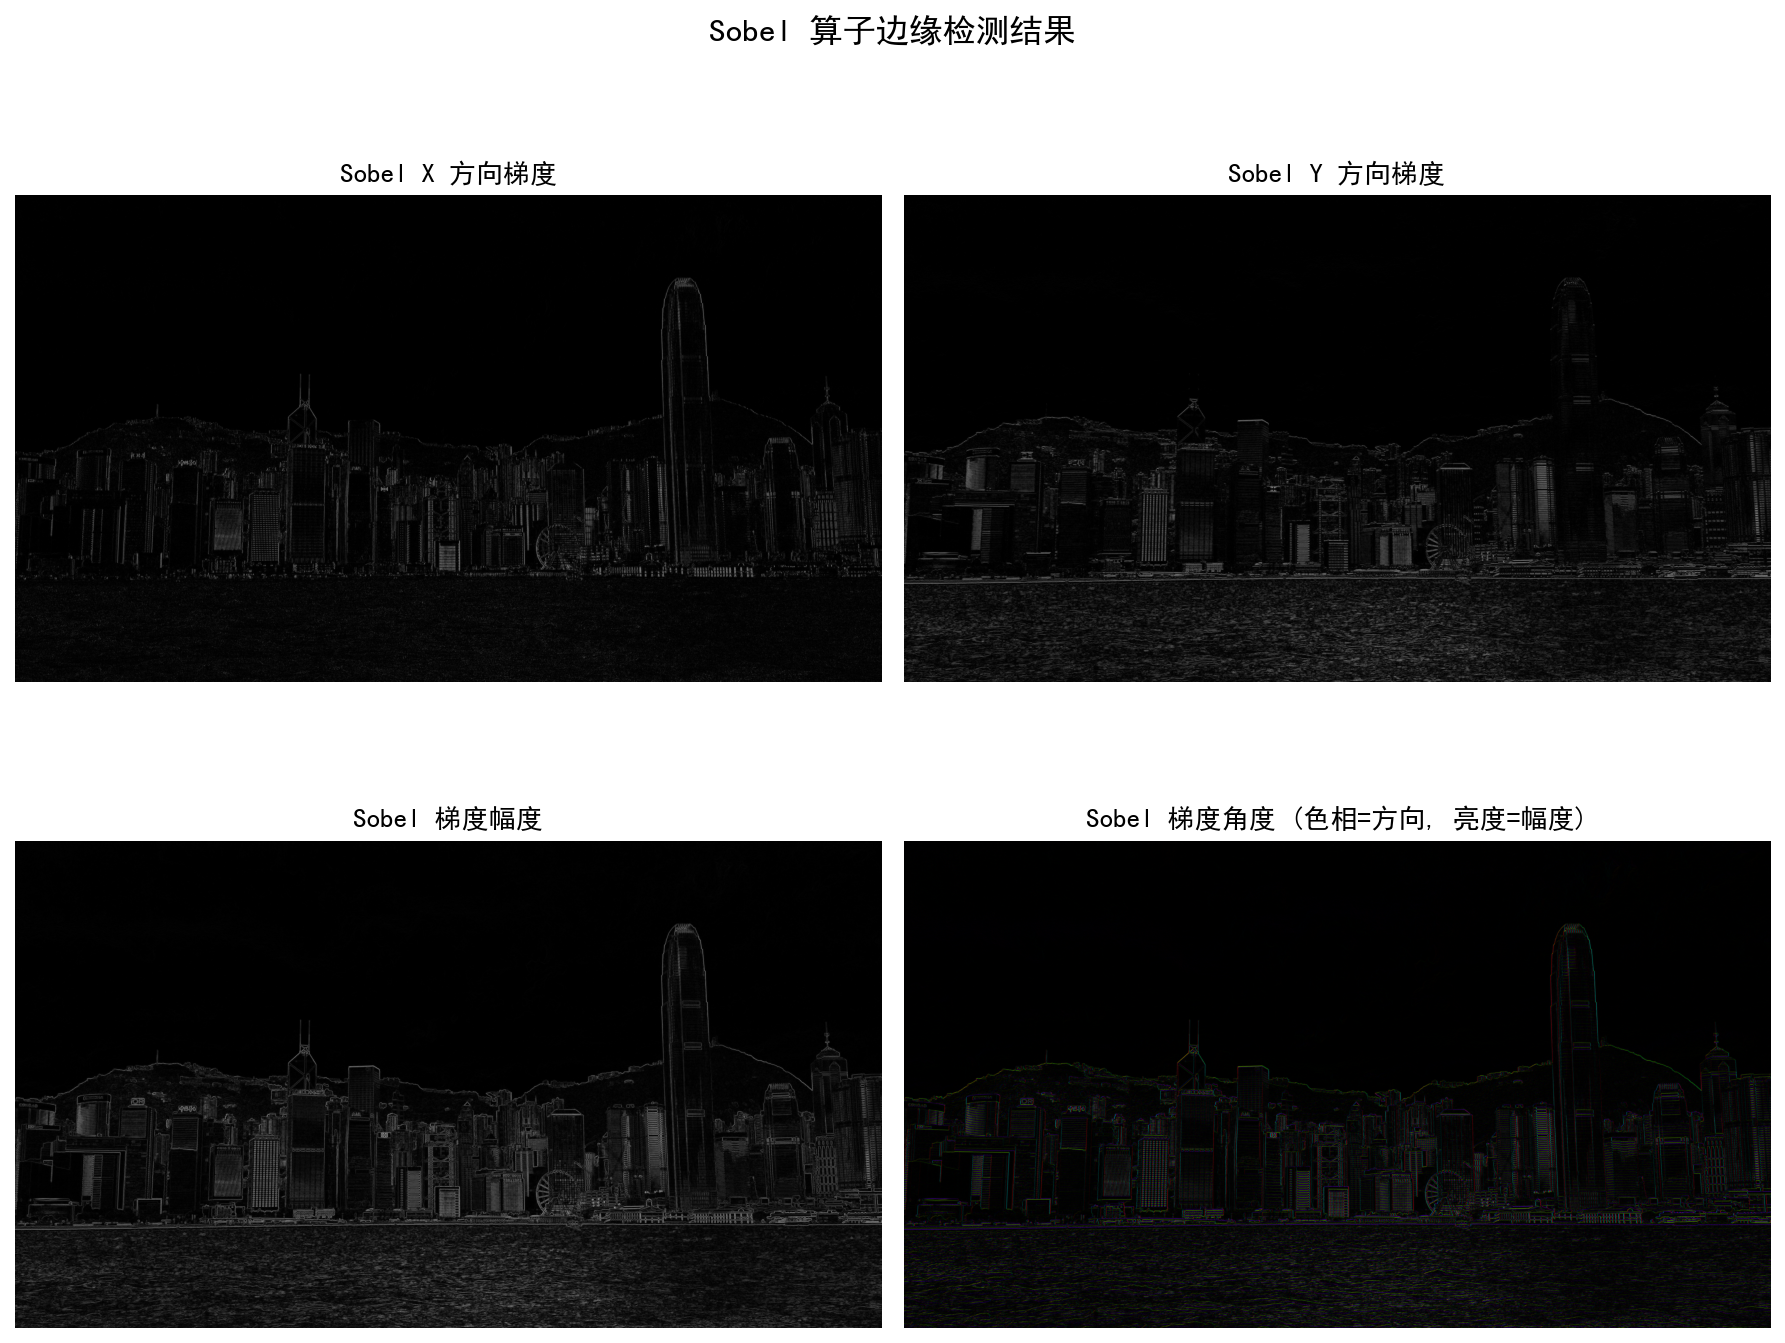
\includegraphics[width=\textwidth]{output_1_sobel.png}
    \caption{Sobel 算子边缘检测——X梯度、Y梯度、梯度幅度、梯度角度}
    \label{fig:sobel}
\end{figure}

\textbf{结果分析：}

\begin{enumerate}[leftmargin=*]
    \item \textbf{X 方向梯度（左上）：}突显了垂直走向的边缘——桥梁的竖直钢索、栏杆支柱。水平边缘（如桥面横梁、水面波纹）在此图中几乎不可见，因为 $G_x$ 对水平方向的亮度变化不敏感。
    \item \textbf{Y 方向梯度（右上）：}突显了水平走向的边缘——桥面轮廓、栏杆横梁、水岸边界。垂直钢索在此图中大幅减弱。X 和 Y 两图互为补充，直观展示了 Sobel 算子的方向选择性。
    \item \textbf{梯度幅度（左下）：}融合了 X 和 Y 两个方向的梯度信息——所有方向的边缘均在图中呈现。由于使用了 L2 范数（$\sqrt{G_x^2+G_y^2}$），边缘强度与方向无关，是对图像"总边缘强度"的最佳估计。
    \item \textbf{梯度角度（右下）：}以颜色编码边缘方向——红色系对应水平边缘（$\theta\approx 0$ 或 $\pm\pi$），青色系对应垂直边缘（$\theta\approx \pm\pi/2$）。亮度代表边缘强度（由幅度调制），暗色区域对应平坦的无边缘区域。
    \item \textbf{整体评价：}Sobel 能有效提取边缘，但边缘线条相对粗糙（宽度约 2--3 像素），且对噪声有一定响应。梯度幅度的动态范围较大，需要归一化才能完整显示。
\end{enumerate}

\subsection{五种算子综合对比}

\begin{figure}[H]
    \centering
    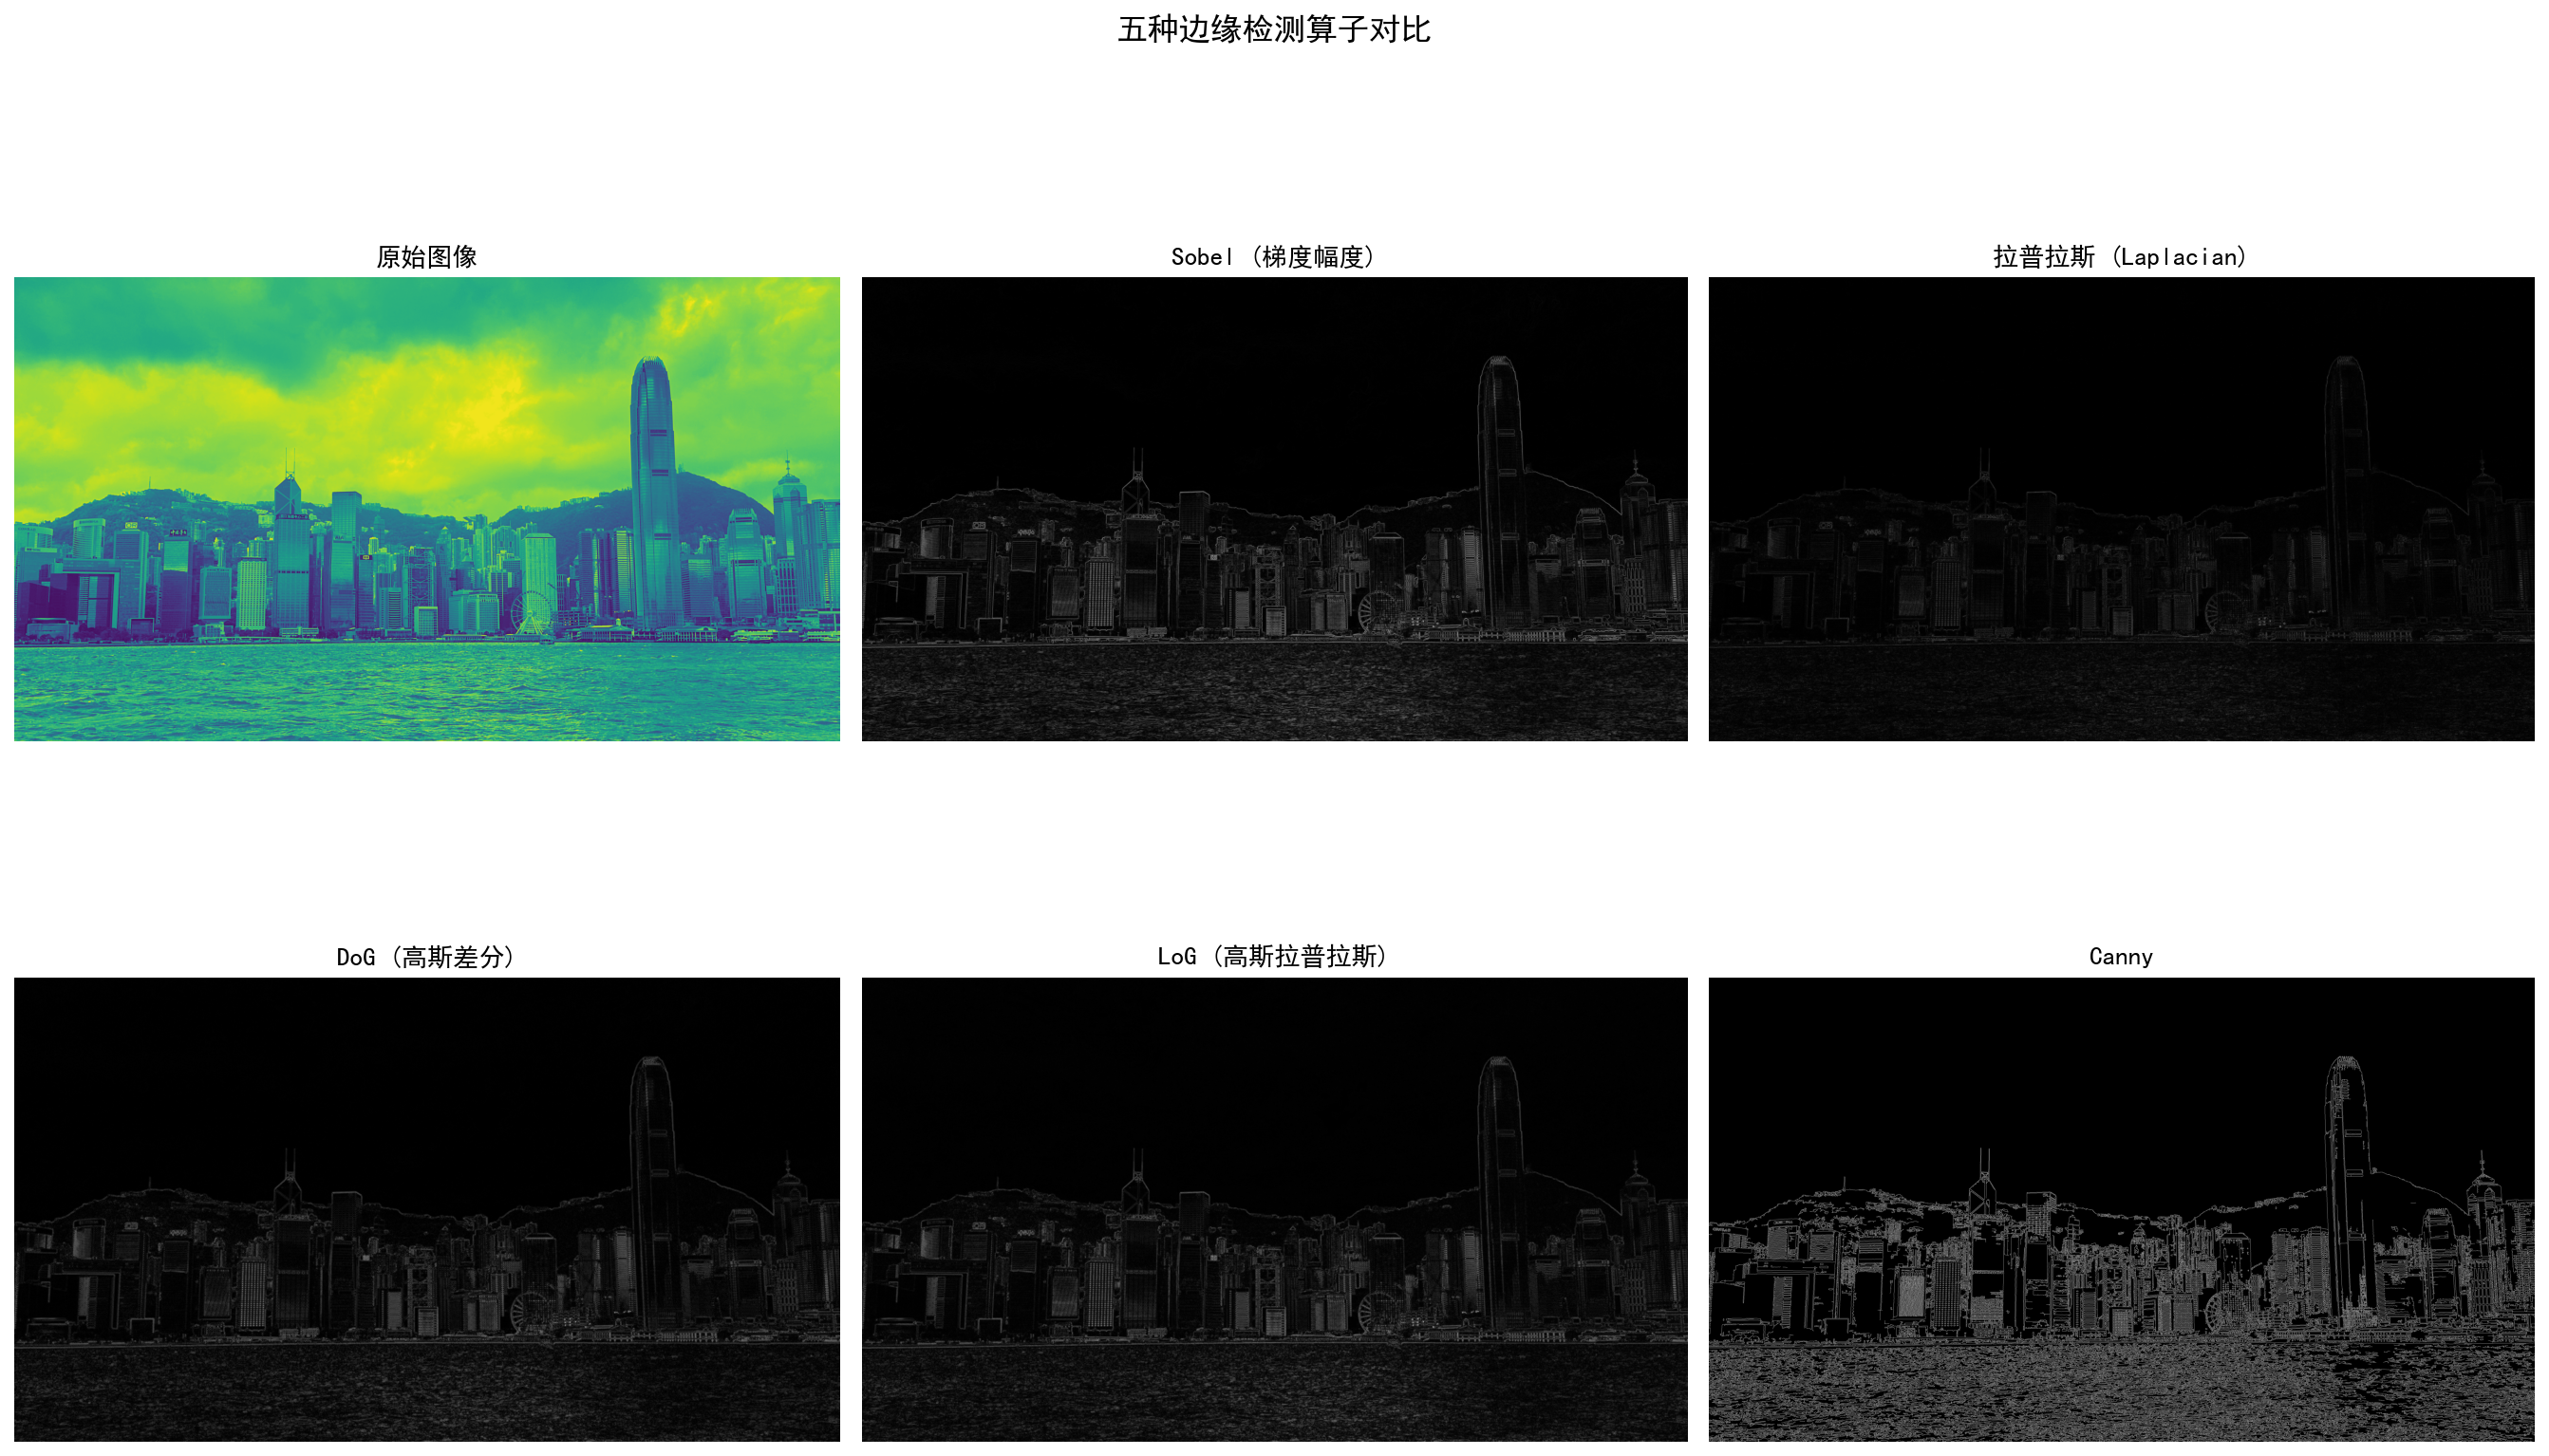
\includegraphics[width=\textwidth]{output_2_all_edges.png}
    \caption{五种边缘检测算子对比（2$\times$3 子图布局）}
    \label{fig:all}
\end{figure}

\textbf{逐算子分析：}

\subsubsection*{Sobel（梯度幅度）}

Sobel 输出的边缘较粗（2--3 像素宽），但能完整捕获图像中的主要结构边缘。钢索、桥塔、栏杆等几何特征均有响应。由于 Sobel 核中隐含了垂直于求导方向的高斯平滑，输出噪声水平可控。主要缺点是无 NMS 后处理导致边缘不够精细。

\subsubsection*{Laplacian}

Laplacian 的输出噪声水平最高——图像平坦区域（天空、水面）出现了大量细密的虚假边缘响应。这是因为二阶导数将噪声放大了约 $O(1/h^2)$ 倍，而原始图像中的传感器噪声即使肉眼不可见，在二阶导数下也会被显著放大。桥梁结构的边缘虽然能检测到，但淹没在噪声中难以区分。\textbf{这直接验证了 Laplacian 算子"必须配合平滑预处理"的结论。}

\subsubsection*{DoG}

DoG 的输出质量明显优于纯 Laplacian——天空和水面的伪边缘大幅减少。$\sigma_1=1.0$ 和 $\sigma_2=2.0$ 的参数组合检测到了该尺度区间内的主要结构边缘（桥梁钢索、桥塔轮廓）。边缘为双边响应（亮暗双边），这是高斯差分操作的固有特征。DoG 在计算效率上的优势使其成为 SIFT 特征检测的标准组件。

\subsubsection*{LoG}

LoG 与 DoG 的视觉效果非常接近，验证了两者的数学等价关系（式 \ref{eq:dog_log}）。LoG 的边缘同样呈现双边响应模式。由于先经过高斯平滑（$\sigma=1.0$），平坦区域的噪声响应被有效抑制。LoG 的边缘定位精度略优于 DoG（LoG 是"真正的"拉普拉斯-高斯核），但差异在实际应用中通常可以忽略。

\subsubsection*{Canny}

Canny 的输出是所有算子中\textbf{最干净、最连续的}：
\begin{itemize}
    \item \textbf{单像素宽度：}非极大值抑制将梯度幅度中的"山脊"细化为精确的单像素边缘——钢索不再是模糊的粗线，而是清晰的细线
    \item \textbf{无背景噪声：}双阈值机制直接丢弃了低梯度区域——平坦的天空和水面完全为黑色，无虚假边缘
    \item \textbf{边缘连续性：}滞后连接确保了边缘片段的完整性——桥梁结构边缘连续不断裂，即使弱边缘部分（水面倒影的边缘）也被保留
    \item \textbf{参数敏感性：}$T_{\text{low}}=50$, $T_{\text{high}}=150$ 在本图效果良好，但不同图像可能需要调节
\end{itemize}

\subsection{综合分析大图}

\begin{figure}[H]
    \centering
    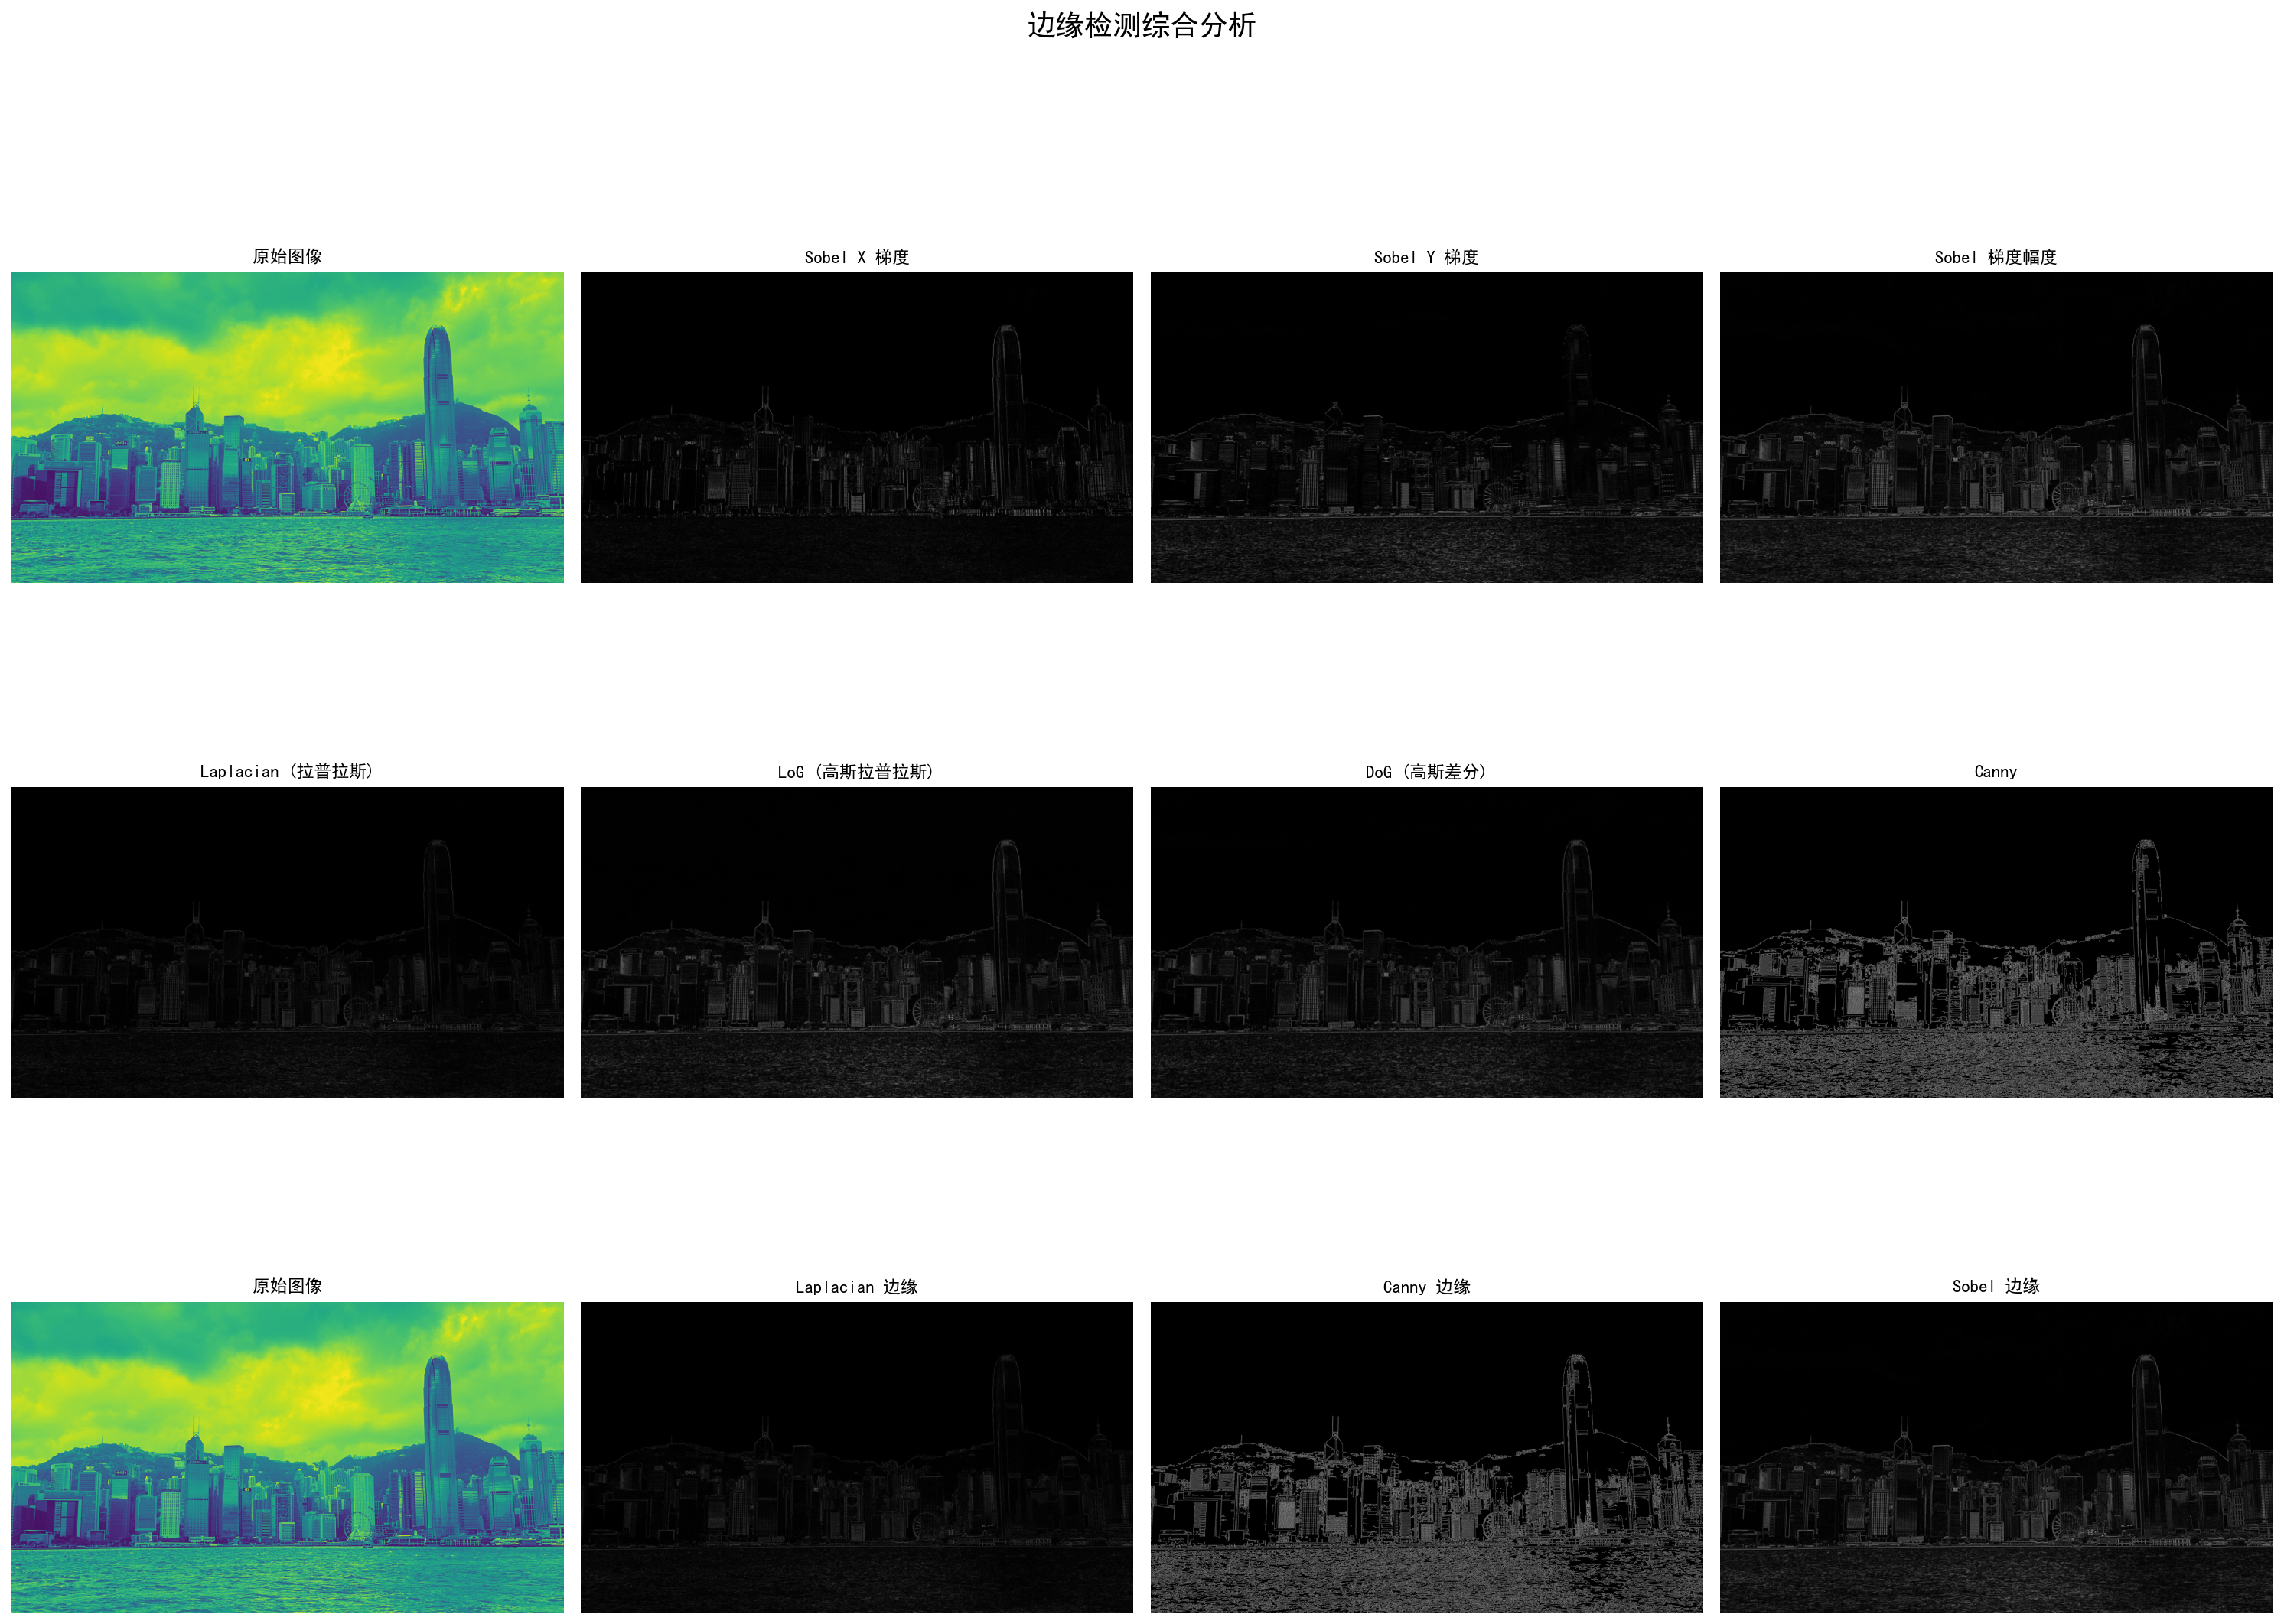
\includegraphics[width=\textwidth]{output_3_comprehensive.png}
    \caption{边缘检测综合分析（3行$\times$4列）}
    \label{fig:comprehensive}
\end{figure}

图 \ref{fig:comprehensive} 将所有结果汇总为 3$\times$4 布局：第一行展示 Sobel 的四个分量输出，第二行对比四种算子的边缘检测结果，第三行以原始图像为参照并列展示三种代表性方法的边缘输出。

\newpage

% ==================== 第五章：讨论 ====================
\section{讨论}

\subsection{一阶导数 vs 二阶导数}

\begin{table}[H]
    \centering
    \caption{一阶与二阶导数边缘检测对比}
    \begin{tabular}{lcc}
        \toprule
        \textbf{特性} & \textbf{一阶导数 (Sobel)} & \textbf{二阶导数 (Laplacian)} \\
        \midrule
        边缘位置 & 梯度幅度极大值 & 二阶导数过零点 \\
        边缘响应 & 单峰 (亮边) & 双边 (亮暗各一条) \\
        方向信息 & 有（可分离 x/y）& 无（各向同性） \\
        对噪声的敏感度 & 中等 & 极高 \\
        计算复杂度 & 两次 $3\times3$ 卷积 & 一次 $3\times3$ 卷积 \\
        典型应用 & 需要方向信息时 & 需配合平滑（LoG） \\
        \bottomrule
    \end{tabular}
\end{table}

一阶导数方法（Sobel）的核心优势是\textbf{方向可分离性}——可以独立获得 X 方向梯度和 Y 方向梯度，进而计算梯度方向，这对 HOG 特征、Canny 的 NMS 等后续处理至关重要。二阶导数方法（Laplacian）的优势是\textbf{各向同性}——对所有方向的边缘产生一致的响应，且过零点定位理论上更精确，但代价是噪声敏感性极高。

\subsection{平滑的必要性}

对比 Laplacian 和 LoG/DoG 的输出可以清晰看到：\textbf{同样的二阶导数算子，有平滑和无平滑的效果天差地别}。这一现象的数学解释为：

\begin{itemize}
    \item 微分运算在频域等价于乘以频率（$\partial/\partial x \leftrightarrow j\omega_x$），二阶导数等价于乘以 $\omega^2$——高频噪声被 $\omega^2$ 倍放大
    \item 高斯平滑在频域等价于乘以 $e^{-\sigma^2\omega^2/2}$，对高频有指数级衰减
    \item 两者级联（LoG）后，频域响应为 $\omega^2 \cdot e^{-\sigma^2\omega^2/2}$——在中间频率处达到峰值，等同于一个\textbf{带通滤波器}
\end{itemize}

因此 LoG/DoG 本质上是带通滤波器——既抑制了低频的缓慢亮度变化（非边缘），又抑制了高频噪声（伪边缘），仅在特定尺度范围内响应真正的边缘。

\subsection{Canny 的优势与代价}

Canny 的输出质量最高，但代价是：
\begin{enumerate}[leftmargin=*]
    \item \textbf{参数敏感：}双阈值 $(T_{\text{low}}, T_{\text{high}})$ 的选择直接影响结果——过高导致边缘断裂，过低导致噪声边缘。通常需要针对不同图像进行调试
    \item \textbf{计算开销：}$O(5\times N)$ ——五阶段流水线比单纯一次卷积更耗时
    \item \textbf{丢失方向信息：}Canny 仅输出二值边缘图（边缘/非边缘），不保留梯度方向和幅度
\end{enumerate}

在实际应用中，如果只需要"哪里是边缘"（如轮廓提取、图像分割），Canny 是最佳选择；如果需要"边缘有多强"和"边缘是什么方向"（如特征描述、立体匹配），Sobel 更为合适。

\subsection{各算子适用场景总结}

\begin{table}[H]
    \centering
    \caption{边缘检测算子适用场景}
    \begin{tabular}{lp{9cm}}
        \toprule
        \textbf{算子} & \textbf{适用场景} \\
        \midrule
        Sobel & 需要方向信息的任务（HOG、光流估计、Canny 的梯度计算阶段） \\
        Laplacian & 仅作为教学对比；或配合平滑用于过零点检测 \\
        LoG & 多尺度边缘检测、斑点检测（Blob Detection） \\
        DoG & SIFT 关键点检测、高效的多尺度边缘提取 \\
        Canny & 通用边缘检测首选、轮廓提取、需要干净二值边缘图的场景 \\
        \bottomrule
    \end{tabular}
\end{table}

\newpage

% ==================== 第六章：总结 ====================
\section{总结}

本实验通过 Python + OpenCV 实现了五种经典边缘检测算子，使用桥梁照片进行了系统的对比实验和理论分析。

\textbf{核心发现：}

\begin{enumerate}[leftmargin=*]
    \item \textbf{Sobel 算子}基于一阶导数，可分离的方向性（X/Y）是其独特优势——能区分水平边缘和垂直边缘，并提供梯度幅度和角度信息。缺点是边缘较粗。
    \item \textbf{Laplacian 算子}基于二阶导数，具有各向同性，但\textbf{对噪声极度敏感}——实验中未平滑的 Laplacian 输出几乎被噪声淹没，直接使用无实用价值。
    \item \textbf{LoG 和 DoG}通过"先平滑再求导"的策略，将二阶导数算子的可用性大幅提升。两者在数学上近似等价（$\sigma_1/\sigma_2\approx 1.6$ 时），DoG 因计算效率更高而成为 SIFT 的标准组件。
    \item \textbf{Canny 算子}凭借非极大值抑制（细化边缘）和双阈值滞后连接（抑制噪声+保持连续性），输出了最干净、最连续的边缘图，是实际工程的首选。
    \item \textbf{边缘检测的本质权衡：}检测率（检出所有真边缘）vs 定位精度（边缘位置精确）vs 抗噪性（不检出伪边缘）——三者不可兼得。高斯平滑的 $\sigma$ 是控制这一权衡的核心参数。
\end{enumerate}

\vspace{0.5cm}
\noindent\textbf{本实验与作业（1）的关联：}
\begin{itemize}
    \item 作业（1）中的高斯平滑和噪声生成为本实验奠定了基础
    \item 作业（1）验证了"中值滤波保边缘、高斯平滑损边缘"——而本实验的 Sobel/Canny 正是利用梯度信息来\textbf{定位}边缘
    \item 两个实验共同揭示了计算机视觉的核心流程：\textbf{预处理（去噪/平滑）→ 特征提取（边缘检测）→ 高层理解}，其中每一步的质量都直接影响后续步骤
\end{itemize}

\newpage

% ==================== 附录 ====================
\appendix
\section{完整源代码 (main.py)}

\lstinputlisting[caption={main.py —— 边缘检测实验完整代码}, label=lst:fullcode]{main.py}

\section{输出文件清单}

\begin{table}[H]
    \centering
    \caption{实验输出文件}
    \begin{tabular}{ll}
        \toprule
        \textbf{文件名} & \textbf{内容} \\
        \midrule
        \texttt{output\_1\_sobel.png} & Sobel 四象限输出（X/Y/幅度/角度） \\
        \texttt{output\_2\_all\_edges.png} & 2$\times$3 五种算子+原始图像对比 \\
        \texttt{output\_3\_comprehensive.png} & 3$\times$4 综合分析大图 \\
        \bottomrule
    \end{tabular}
\end{table}

\section{运行说明}

\begin{lstlisting}[language=bash, caption={运行命令}]
pip install -r requirements.txt
python main.py input_photo.jpg
\end{lstlisting}

生成的 3 张 PNG 输出图将保存在当前目录。

\end{document}
